\documentclass[11pt,a4paper]{article}
\usepackage[margin=25mm,headheight=15pt]{geometry}
\usepackage[T1]{fontenc}
\usepackage{newtxtext}
\usepackage{mathtools,amsthm}
\usepackage{newtxmath}
\usepackage{microtype,graphicx,booktabs,array,longtable}
\usepackage{enumitem,fancyhdr,xcolor,xurl,needspace}
\usepackage[colorlinks=true,linkcolor=blue!35!black,citecolor=blue!35!black,urlcolor=blue!40!black]{hyperref}
\usepackage[nameinlink,noabbrev]{cleveref}
\setlength{\parskip}{4pt}
\setlength{\parindent}{1.25em}
\setlength{\emergencystretch}{2em}
\allowdisplaybreaks[2]
\pagestyle{fancy}
\fancyhf{}
\fancyhead[L]{\small Spectral inversion and direct optimal truncation}
\fancyhead[R]{\small ProveIt research extension}
\fancyfoot[C]{\thepage}
\renewcommand{\headrulewidth}{0.3pt}
\newtheorem{theorem}{Theorem}[section]
\newtheorem{proposition}[theorem]{Proposition}
\newtheorem{lemma}[theorem]{Lemma}
\newtheorem{corollary}[theorem]{Corollary}
\theoremstyle{definition}
\newtheorem{definition}[theorem]{Definition}
\newtheorem{remark}[theorem]{Remark}
\newtheorem{problem}{Research problem}
\numberwithin{equation}{section}
\newcommand{\dd}{\mathop{}\!\mathrm{d}}
\newcommand{\ii}{\mathrm{i}}
\newcommand{\ee}{\mathrm{e}}
\newcommand{\C}{\mathbb C}
\newcommand{\R}{\mathbb R}
\newcommand{\N}{\mathbb N}
\newcommand{\Oh}{\mathcal O}
\newcommand{\E}{\mathbb E}
\newcommand{\Borel}{\mathcal B}
\newcommand{\cformal}{\mathcal C}
\newcommand{\U}{\mathcal U}
\newcommand{\repo}{\textit{ProveIt}}
\newcommand{\rising}[2]{(#1)_{#2}}
\DeclareMathOperator{\Res}{Res}
\hypersetup{pdftitle={A Spectral Representation for the Inverse Digamma Function},pdfauthor={Research article prepared for Vladimir Reshetnikov},pdfsubject={Direct optimal truncation, eventual enveloping, and inverse Borel boundary singularities}}
\begin{document}
% ed. (2026-09-29): no page anchor on the title page, which otherwise shares its page number with the
% next page (pdfTeX "duplicate destination" warning); the same device the Stokes-transport package uses.
\hypersetup{pageanchor=false}
\begin{titlepage}
\vspace*{9mm}
\noindent{\large\scshape Transseries, asymptotic inversion, and resurgence}\par
\vspace{10mm}
\noindent{\huge\bfseries\raggedright A Spectral Representation\\[2mm] for the Inverse Digamma\\[2mm] Function\par}
\vspace{7mm}
\noindent{\Large Direct optimal truncation, eventual enveloping,\newline and inverse Borel boundary singularities\par}
\vspace{10mm}
\noindent Research article prepared for Vladimir Reshetnikov\par
\noindent 29 September 2026\par
\vspace{8mm}\hrule\vspace{5mm}
\begin{abstract}
The \repo\ manuscript on inverse harmonic transseries leaves open the sharp remainder of a \emph{direct} inverse partial sum, as distinct from the inverse of a truncated forward expansion. We resolve this question in the large-positive-variable regime, including every algebraic correction to the leading exponential error. For the exterior inverse defined by
$\psi(W(X)+\tfrac12)=\log X$, put
$S_M(X)=X+\sum_{n=1}^M h_nX^{1-2n}$ and
$\sigma=M+1-\pi X$. Uniformly for bounded $\sigma$,
\[
 S_M-W=(-1)^M\sqrt X\,\ee^{-2\pi X}
 \left[1+\frac1X\left\{\frac{2\sigma^2-3\sigma+7/12}{2\pi}
                       -\frac\pi{12}\right\}+\Oh(X^{-2})\right].
\]
The proof constructs an exact positive spectral density
$\rho(t)=-\Re W(\ii t)$ for sufficiently large $t$. Cauchy's formula represents $W-X$ as a negative Stieltjes-type integral of this density plus a genuinely convergent Laurent correction. This representation also proves eventual strict enveloping, an elementary cosine representation of the inverse Borel transform, and every logarithmic coefficient in its one-sided boundary expansions at $\pm2\pi\ii$. A general theorem transfers an exponentially small boundary-phase defect into inverse late coefficients and an optimal-truncation constant. Exact finite algebra, 240-digit tests, and an independent contour calculation accompany the proofs.
\end{abstract}
\vspace{3mm}
\noindent\textbf{Status and scope.} The article supplies conventional mathematical proofs and reproducible finite checks. It does not claim a new Lean formalization, global priority, global enveloping at every argument and order, or complete continuation data on every Borel sheet. Classical inverse-digamma coefficient asymptotics and existing nonlinear resurgence theory are explicitly credited.
\vfill
\noindent\small Inspected repository checkpoint:\par
\noindent\small\texttt{5804c7aff9955e6cbc09be2a71a295a07b238bc9}.\par
\end{titlepage}
\hypersetup{pageanchor=true}
\begingroup\small\setlength{\parskip}{0pt}\tableofcontents\endgroup
\newpage

\section{The question, the contribution, and its boundaries}
\label{sec:intro}

\subsection{Two approximations that must not be confused}
Let $\psi=\Gamma'/\Gamma$ be the digamma function. The centered harmonic inverse is the real large-$X$ solution of
\begin{equation}
 F(W(X))=\log X,\qquad F(w)=\psi(w+\tfrac12).
 \label{eq:normalization}
\end{equation}
It translates into the inverse of the continuously interpolated harmonic numbers by
\begin{equation}
 H(x)=\psi(x+1)+\gamma,\qquad
 H^{-1}(y)=W(\ee^{y-\gamma})-\tfrac12.
 \label{eq:harmonic}
\end{equation}
The formal inverse has an odd Laurent expansion
\begin{equation}
 W(X)\sim X+\sum_{n\ge1}h_nX^{1-2n}.
 \label{eq:formal-intro}
\end{equation}
There are two natural ways to use it computationally. One may truncate \eqref{eq:formal-intro} directly, obtaining $S_M$. Alternatively, one may truncate the expansion of $F$ and solve the resulting forward equation, obtaining $u_M$. Even when both constructions have the same exponentially small leading error, their first corrections need not agree.

The repository's \emph{Exponential Accuracy and Stokes Transport for Inverse Harmonic Transseries} \cite{prior} proves the forward-truncation-inverse result. Its research discussion explicitly withholds the corresponding claim for $S_M$ and proposes an analytic inverse representation as a possible route. The present article implements that route without assuming global univalence of the inverse and without discarding the contribution from a fixed inner contour.

\subsection{What is proved}
The central analytic construction is an exact representation
\begin{equation}
 W(X)-X=E_R(X)-\frac{2X}{\pi}
      \int_R^\infty\frac{\rho(t)}{X^2+t^2}\,\dd t,
 \qquad \rho(t)=-\Re W(\ii t)>0,
 \label{eq:intro-spectral}
\end{equation}
where $R$ is sufficiently large and $E_R$ is represented by a convergent odd Laurent series for $|X|>R$. The density is determined by the same exterior inverse branch as the real function. It is not an auxiliary density fitted to coefficients.

From \eqref{eq:intro-spectral} we obtain four connected conclusions. First, a finite geometric identity gives the \emph{exact} direct-truncation remainder, including the inner-contour correction. Second, its gamma-moment analysis proves a sharp exponential expansion to every fixed relative algebraic order. Third, the positivity of the spectral part dominates the convergent correction uniformly at sufficiently high truncation orders, giving consecutive-partial-sum brackets. Fourth, the ordinary Borel transform is a cosine transform of the same density, up to an entire function. Its nearest one-sided singular expansions therefore follow from the density asymptotics.

The detailed statements are \cref{thm:spectral,thm:remainder,thm:enveloping,thm:optimal,thm:borel,thm:boundary}. The general transfer theorem in \cref{sec:general} isolates the part of the argument that is not specific to the digamma function.

\subsection{Existing work and novelty positioning}
Coefficient formulas for inverse-digamma expansions and their large-order asymptotics are not new: Issaka studied them in the context of Ramanujan's inverse-digamma approximation \cite{issaka}. The repository also contains the centered coefficient formula and complete late-order analysis \cite{prior,companion}. We rederive their leading consequences from the spectral representation as a consistency check, not as a priority claim.

Contour representations for asymptotic reversion and enveloping estimates have important precedents. In particular, Nemes proves enveloping results for reverted cylinder- and Airy-zero expansions using analytic representations \cite{nemes}. Our construction is specialized to the centered inverse digamma function, whose reflection identity produces a particularly explicit boundary-phase defect. General algebraic treatment of factorial asymptotics is developed by Borinsky \cite{borinsky}, while nonlinear resurgent closure and summability under inversion are supplied by Sauzin \cite{sauzin}. The new work claimed relative to the inspected repository is the exact spectral decomposition, the direct-inverse remainder theorem, the eventual uniform envelopes, the direct-versus-forward subleading comparison, and the explicit one-sided Borel boundary data derived from that decomposition.

A targeted literature check does not establish worldwide priority. These claims should be read as proved research contributions offered for independent mathematical review, not as assertions of publication status. The exact repository paths, commit, inspected boundary, and computational limitations are recorded in \cref{app:provenance}.

\section{The exterior inverse and its formal coefficients}
\label{sec:inverse}

\subsection{A sector larger than the right half-plane}
Fix $0<\varepsilon<\pi/4$. We use principal logarithms and a sector
\[
 \Sigma_{\varepsilon,R}
 =\{z:|z|>R,\ |\arg z|<\pi/2+\varepsilon\}.
\]
All uniform asymptotic statements on this sector may be interpreted on a slightly smaller closed sector; the initial sector can always be chosen slightly larger. This convention leaves room for disks and Cauchy derivative estimates.

The classical sectorial digamma expansion \cite[\S5.11]{dlmf} gives
\begin{equation}
 F(w)=\log w+C(w),\qquad
 C(w)\sim\sum_{j\ge1}c_jw^{-2j},\qquad
 c_j=-\frac{B_{2j}(1/2)}{2j}.
 \label{eq:centered}
\end{equation}
In particular, $C(w)=\Oh(w^{-2})$, $C'(w)=\Oh(w^{-3})$, and
$F''(w)=\Oh(w^{-2})$ uniformly. The even-power form follows either by shifting the standard digamma expansion or by the Bernoulli-polynomial form of the shifted expansion. The same uniform expansions may be differentiated on smaller sectors by Cauchy's formula.

\begin{lemma}[Exterior inverse branch]
\label{lem:inverse}
For sufficiently large $R$, there is a unique holomorphic solution $W$ on $\Sigma_{\varepsilon,R}$ satisfying
\begin{equation}
 F(W(z))=\log z,\qquad W(z)=z+\Oh(z^{-1}).
 \label{eq:branch}
\end{equation}
Uniqueness means uniqueness among solutions in a fixed disk $|w-z|\le K/|z|$ for a suitable fixed $K$. The branch obeys
$W(\overline z)=\overline{W(z)}$, and has the expansion \eqref{eq:formal-intro} to every fixed order, uniformly on smaller sectors.
\end{lemma}
\begin{proof}
Rewrite the equation as
\[
 w=T_z(w):=z\exp(-C(w)).
\]
For $|w-z|\le K/|z|$ and large $|z|$, the estimate on $C$ makes $T_z$ map this disk into itself when $K$ is large enough. Its derivative is
$-z\exp(-C(w))C'(w)=\Oh(|z|^{-2})$, uniformly. It is therefore a contraction. The fixed point depends holomorphically on $z$, by the holomorphic implicit function theorem or locally uniform convergence of the iterates. Local solutions agree on overlaps by the same uniqueness.

The fixed-point equation implies the original logarithmic equation: both $\log(w/z)$ and $-C(w)$ are small, so the ambiguity by $2\pi\ii$ is absent. Conjugation symmetry follows from that of $F$ and uniqueness. Formal coefficient cancellation constructs the inverse to any fixed order. Substituting its finite truncation into the fixed-point equation leaves an error of the next required order, and the uniform contraction estimate bounds the difference from the exact fixed point. Equivalently, the derivative of $F$ is $z^{-1}(1+\Oh(z^{-2}))$ in the relevant disk. This gives the stated uniform asymptotic expansion.
\end{proof}

\begin{remark}[No global inverse theorem is being assumed]
The lemma provides exactly the branch needed on the right half-plane outside a disk and on both imaginary boundary rays. It makes no assertion about critical values or singularities inside that disk. Keeping the inner contour in \eqref{eq:intro-spectral} is what permits us to avoid those global questions.
\end{remark}

\subsection{The finite coefficient formula}
Put $\cformal(z)=\sum_{j\ge1}c_jz^j$. The formal defining equation is
\begin{equation}
 \log(W/X)+\cformal(W^{-2})=0.
 \label{eq:formal-equation}
\end{equation}
The coefficient formula already used in the repository is
\begin{equation}
 h_n=-\frac1{2n-1}[z^n]\exp\bigl((2n-1)\cformal(z)\bigr).
 \label{eq:h-coeff}
\end{equation}
For completeness, set $v=1/W$ and $t=1/X$. Then
$v=t\exp(\cformal(v^2))$. Formal Lagrange inversion, or a formal-residue change of variable, gives
\[
 [t^{2n-1}]\frac1{v(t)}
 =-\frac1{2n-1}[u^{2n}]\exp\bigl((2n-1)\cformal(u^2)\bigr),
\]
which proves \eqref{eq:h-coeff}. Only finite coefficient extraction is involved at each $n$.

The first values are
\begin{align}
 c_1&=\frac1{24},&c_2&=-\frac7{960},&c_3&=\frac{31}{8064},\label{eq:c-first}\\
 h_1&=-\frac1{24},&h_2&=\frac3{640},&h_3&=-\frac{1525}{580608},\notag\\
 h_4&=\frac{615881}{199065600},&&h_5=-\frac{3058641}{504627200}.
 \label{eq:h-first}
\end{align}
These values fix the normalization and signs used throughout the article. In particular, the first direct inverse correction is negative.

\section{Reflection creates an exponentially small spectral density}
\label{sec:density}

\subsection{The boundary-phase defect}
For $v>0$, write
\begin{equation}
 F(\ii v)=A(v)+\ii B(v).
 \label{eq:AB}
\end{equation}
The digamma reflection identity \cite[\S5.5(ii)]{dlmf} gives the exact formulas
\begin{equation}
 B(v)=\frac\pi2\tanh(\pi v),\qquad
 J(v):=\frac\pi2-B(v)=\frac{\pi}{\ee^{2\pi v}+1}.
 \label{eq:phase-defect}
\end{equation}
Indeed, the two arguments $1/2\pm\ii v$ are conjugate, so their digamma difference is twice the imaginary part. Substitution into
$\psi(z)-\psi(1-z)=-\pi\cot(\pi z)$ yields \eqref{eq:phase-defect}.

The differentiated centered expansion gives
\begin{equation}
 A(v)\sim\log v+\sum_{j\ge1}(-1)^jc_jv^{-2j},\quad
 A'(v)=v^{-1}+\Oh(v^{-3})>0,
 \label{eq:A-expansion}
\end{equation}
and $B'(v)=\Oh(\ee^{-2\pi v})$. Thus for large $t$ the real equation
\begin{equation}
 A(v(t))=\log t
 \label{eq:v-definition}
\end{equation}
has a unique solution $v(t)=t+\Oh(t^{-1})$. Differentiation gives
\begin{equation}
 \frac1{A'(v(t))}=t\,v'(t).
 \label{eq:v-derivative}
\end{equation}
The exact difference between $F(\ii v(t))$ and the desired value $\log(\ii t)$ is $\ii J(v(t))$. It is this exponentially small mismatch, not an algebraic correction, that displaces the inverse off the imaginary axis.

\begin{theorem}[Positive density and its complete algebraic amplitude]
\label{thm:density}
Let $a=2\pi$. For all sufficiently large $t$, define
\begin{equation}
 \rho(t)=-\Re W(\ii t).
 \label{eq:rho}
\end{equation}
Then $\rho(t)>0$ and
\begin{equation}
 \rho(t)=\pi t v'(t)\ee^{-a v(t)}+\Oh(t^3\ee^{-2at}).
 \label{eq:rho-v}
\end{equation}
For every fixed integer $J\ge1$,
\begin{equation}
 \rho(t)=\pi t\ee^{-at}
 \left(\sum_{j=0}^{J-1}d_jt^{-j}+\Oh_J(t^{-J})\right).
 \label{eq:rho-asympt}
\end{equation}
All $d_j$ are obtained by the formal identity
\begin{equation}
 V'(t)\exp[-a(V(t)-t)]=\sum_{j\ge0}d_jt^{-j},\qquad
 V(t)=t+\sum_{n\ge1}(-1)^nh_nt^{1-2n}.
 \label{eq:d-algorithm}
\end{equation}
In particular,
\begin{equation}
 d_0=1,\qquad d_1=-\frac\pi{12},\qquad
 d_2=\frac{\pi^2}{288}-\frac1{24}.
 \label{eq:d-first}
\end{equation}
\end{theorem}
\begin{proof}
Set $v=v(t)$ and $W(\ii t)=\ii v+\delta$. Differentiating \eqref{eq:AB} gives
\begin{equation}
 F'(\ii v)=B'(v)-\ii A'(v).
 \label{eq:Fprime-boundary}
\end{equation}
The local inverse of $F$ near $\ii v$ has first derivative $\Oh(v)$ and second derivative $\Oh(v)$, because $F'=\Theta(v^{-1})$ and $F''=\Oh(v^{-2})$. For clarity about uniformity, scale $w=\ii v+vh$. On a fixed sufficiently small $h$-disk, $F(\ii v+vh)-F(\ii v)$ is uniformly close, with derivatives, to $\log(1+h/\ii)$. Rouch\'e's theorem on a smaller disk therefore gives a unique local inverse on a value disk of radius independent of $v$. On this inverse disk its first two derivatives have the stated $\Oh(v)$ bounds. Taylor's theorem for that local inverse, applied to the value increment $\ii J(v)$, yields
\begin{equation}
 \delta=\frac{\ii J(v)}{B'(v)-\ii A'(v)}+\Oh(vJ(v)^2).
 \label{eq:delta}
\end{equation}
The inverse obtained this way is the branch from \cref{lem:inverse}, by its uniqueness near $\ii t$.

Taking minus the real part of \eqref{eq:delta} gives
\begin{equation}
 \rho(t)=\frac{J(v)A'(v)}{A'(v)^2+B'(v)^2}+\Oh(vJ(v)^2).
 \label{eq:rho-exact-leading}
\end{equation}
The leading term is positive and asymptotic to $\pi v\ee^{-av}$; the error divided by that term tends to zero. This proves eventual positivity. Using
$J(v)=\pi\ee^{-av}+\Oh(\ee^{-2av})$,
$B'(v)=\Oh(\ee^{-av})$, \eqref{eq:v-derivative}, and $v=t+\Oh(t^{-1})$ proves the conservative error bound \eqref{eq:rho-v}.

The implicit real inversion in \eqref{eq:v-definition}, with the differentiated expansion \eqref{eq:A-expansion}, gives the formal series $V$ and its differentiated expansion to every fixed order. This is a consequence of the analytic derivative estimates above; it is not a differentiation of an arbitrary unqualified real asymptotic relation. Substitution into \eqref{eq:rho-v} proves \eqref{eq:rho-asympt}, since its exponentially smaller error is smaller than every requested relative power of $t^{-1}$. Finally,
$V=t+1/(24t)+\Oh(t^{-3})$ and
$V'=1-1/(24t^2)+\Oh(t^{-4})$, giving \eqref{eq:d-first}.
\end{proof}

\begin{remark}[The sign is a consequence of reflection]
The density is not postulated to be positive because the first few $h_n$ alternate. Positivity comes from the positive defect $J$, the positive derivative $A'$, and an exponentially smaller nonlinear error. This logical order is essential for the later enveloping theorem.
\end{remark}

\section{An exact dispersion formula with a convergent inner correction}
\label{sec:spectral}

Choose $R$ large enough that the exterior inverse exists on a neighborhood of the closed right half-plane outside $|z|=R$, and that $\rho(t)>0$ for $t\ge R$. Define a piecewise holomorphic exterior function by
\begin{equation}
 \U(z)=
 \begin{cases}
 W(z)-z,&\Re z>0,\\
 -W(-z)-z,&\Re z<0.
 \end{cases}
 \label{eq:piecewise}
\end{equation}
Its boundary values on the imaginary rays are taken from the respective half-planes. It is odd, respects conjugation, and is uniformly $\Oh(1/z)$ at infinity. By conjugation symmetry,
\begin{equation}
 \U_R(\ii t)-\U_L(\ii t)
 =\U_R(-\ii t)-\U_L(-\ii t)=-2\rho(t),\qquad t\ge R.
 \label{eq:jump}
\end{equation}
The subscripts indicate right and left limits, not upper and lower limits.

\begin{theorem}[Exact spectral decomposition]
\label{thm:spectral}
For $\Re z>0$ and $|z|>R$,
\begin{equation}
 W(z)-z=E_R(z)-\frac{2z}{\pi}
       \int_R^\infty\frac{\rho(t)}{z^2+t^2}\,\dd t,
 \label{eq:spectral}
\end{equation}
where
\begin{equation}
 E_R(z)=\frac1{2\pi\ii}\oint_{|\zeta|=R}^{\rm ccw}
           \frac{\U(\zeta)}{z-\zeta}\,\dd\zeta
       =\sum_{n\ge1}e_nz^{1-2n}.
 \label{eq:core}
\end{equation}
The contour integral uses the right and left definitions on the corresponding semicircles. Its Laurent series converges for $|z|>R$. If
$K_R=R\sup_{|\zeta|=R}|\U(\zeta)|$, with the supremum taken over those arcs, then
\begin{equation}
 |e_n|\le K_R R^{2n-2}.
 \label{eq:e-bound}
\end{equation}
\end{theorem}
\begin{proof}
Apply Cauchy's formula to the right and left portions of the annulus $R<|\zeta|<L$, avoiding the imaginary seams by parallel contours, and add the two formulas. The left portion contains no pole at the evaluation point $z$; the right portion contains the usual one. The outer-circle contribution tends to zero as $L\to\infty$, because the kernel is $\Oh(L^{-1})$, $\U=\Oh(L^{-1})$, and the contour length is $\Oh(L)$.

The inner boundary is clockwise. Changing it to counterclockwise gives exactly the first expression in \eqref{eq:core}. On the upper seam, the right boundary is traversed downward, so the two seam contributions involve the negative of the right-minus-left jump. Inserting \eqref{eq:jump} yields
\[
 \frac1\pi\int_R^\infty\frac{\rho(t)}{\ii t-z}\,\dd t
 +\frac1\pi\int_R^\infty\frac{\rho(t)}{-\ii t-z}\,\dd t
 =-\frac{2z}{\pi}\int_R^\infty\frac{\rho(t)}{z^2+t^2}\,\dd t.
\]
The exponential decay in \cref{thm:density} justifies all infinite seam limits. Small joining arcs at the endpoints of the seams have vanishing contributions. This proves \eqref{eq:spectral} with its sign.

Expand $(z-\zeta)^{-1}$ uniformly on the inner circle. Oddness of $\U$ removes the even inverse powers, and
\begin{equation}
 e_n=\frac1{2\pi\ii}\oint_{|\zeta|=R}^{\rm ccw}
              \U(\zeta)\zeta^{2n-2}\,\dd\zeta.
 \label{eq:e-contour}
\end{equation}
The contour-length estimate gives \eqref{eq:e-bound}. Conjugation symmetry makes all $e_n$ real.
\end{proof}

\subsection{Why the correction cannot be suppressed}
The function $E_R$ records the contribution from a fixed bounded region that the exterior construction deliberately excludes. It is convergent, but not necessarily zero. Declaring the full inverse to be a Stieltjes function would require an additional global analytic argument not supplied here. The exact statement is a Stieltjes-type representation \emph{modulo a convergent Laurent function}.

Changing $R$ changes the spectral integral by a finite-interval integral. That difference has a convergent Laurent expansion for $|z|$ larger than both cutoffs and is absorbed into $E_R$. Thus the full expression is independent of the cutoff, as it must be. This also explains why the factorial late coefficients and nearest Borel singular data are unaffected by changing $R$.

\subsection{Exact moments for the inverse coefficients}
\begin{corollary}[Moment decomposition]
\label{cor:moments}
For every $n\ge1$,
\begin{equation}
 h_n=e_n+\frac{2(-1)^n}{\pi}
                 \int_R^\infty\rho(t)t^{2n-2}\,\dd t.
 \label{eq:h-moment}
\end{equation}
Consequently, for each fixed $J\ge1$,
\begin{equation}
 \frac{h_n}{2(-1)^n\Gamma(2n)/a^{2n}}
 =\sum_{j=0}^{J-1}d_ja^j\frac{\Gamma(2n-j)}{\Gamma(2n)}
       +\Oh_J(n^{-J}),\qquad a=2\pi.
 \label{eq:late}
\end{equation}
\end{corollary}
\begin{proof}
Apply a finite geometric expansion to the kernel in \eqref{eq:spectral}. The exponential decay of $\rho$ makes every resulting moment finite and bounds the fixed-order remainder. Uniqueness of the asymptotic coefficients from \cref{lem:inverse} gives \eqref{eq:h-moment}.

Insert \eqref{eq:rho-asympt} into the moment integral. Replacing the lower endpoint by zero in each monomial term changes it by a geometrically bounded quantity in $n$. The density remainder contributes at most a constant times $\Gamma(2n-J)/a^{2n-J}$. The inner coefficients and fixed-interval contributions are negligible compared with every such factorial quantity. Dividing by the leading moment proves \eqref{eq:late}.
\end{proof}
The leading equivalent in \eqref{eq:late} is already known \cite{issaka,prior}. The point here is that the same exact representation producing it also controls the actual direct-truncation remainder.

\section{Exact direct remainders and eventual strict enveloping}
\label{sec:remainder}

For an integer $M\ge0$, define
\begin{equation}
 S_M(X)=X+\sum_{n=1}^M h_nX^{1-2n},\qquad
 \mathcal E_{R,M}(X)=E_R(X)-\sum_{n=1}^M e_nX^{1-2n}.
 \label{eq:partial-sums}
\end{equation}
An empty sum is zero. The following identity, not a late-coefficient estimate, is the basis of the sharp remainder theorem.

\begin{theorem}[Exact direct-inverse remainder]
\label{thm:remainder}
For real $X>R$ and $M\ge0$,
\begin{equation}
 W(X)-S_M(X)=\mathcal E_{R,M}(X)
 +\frac{2(-1)^{M+1}}{\pi X^{2M+1}}
       \int_R^\infty\frac{\rho(t)t^{2M}}{1+(t/X)^2}\,\dd t.
 \label{eq:exact-remainder}
\end{equation}
Moreover,
\begin{equation}
 |\mathcal E_{R,M}(X)|\le
 \frac{K_R R^{2M}X^{-2M-1}}{1-(R/X)^2}.
 \label{eq:core-tail-bound}
\end{equation}
\end{theorem}
\begin{proof}
Use the finite identity
\[
 \frac1{1+u}=\sum_{k=0}^{M-1}(-u)^k+\frac{(-u)^M}{1+u}
\]
with $u=(t/X)^2$ in \eqref{eq:spectral}. Formula \eqref{eq:h-moment} identifies the finite coefficients and gives \eqref{eq:exact-remainder}. This is valid even when the finite geometric polynomial is large; no convergence of an infinite geometric series is used under the integral. Summing the geometric majorant from \eqref{eq:e-bound} proves \eqref{eq:core-tail-bound}.
\end{proof}

\begin{theorem}[Uniform eventual strict enveloping]
\label{thm:enveloping}
There are constants $R>0$ and an integer $M_0$ such that for every real $X\ge2R$ and every integer $M\ge M_0$,
\begin{equation}
 (-1)^{M+1}\bigl(W(X)-S_M(X)\bigr)>0.
 \label{eq:sign}
\end{equation}
In particular, $W(X)$ lies strictly between $S_M(X)$ and $S_{M+1}(X)$, and
\begin{equation}
 0<|W(X)-S_M(X)|<|h_{M+1}|X^{-2M-1}.
 \label{eq:envelope-bound}
\end{equation}
The constants are existential in this proof; no numerical value for a globally valid $R$ or $M_0$ is asserted.
\end{theorem}
\begin{proof}
Increase $R$ so that $\rho(t)\ge c\,t\ee^{-at}$ for $t\ge R$, where $c>0$ and $a=2\pi$. Put $k=2M+2$. For all sufficiently large $M$, the interval $[k/(2a),2k/a]$ lies above $R$. A gamma random variable $U$ of shape $k$ and unit rate has mean $k$ and variance $k$. Chebyshev's inequality shows that
$\mathbb P(k/2\le U\le2k)\ge1/2$ once $k$ is sufficiently large. It follows that
\begin{equation}
 \int_R^\infty\frac{\rho(t)t^{2M}}{1+(t/X)^2}\,\dd t
 \ge \frac{c\,\Gamma(k)}{2a^k}
       \frac1{1+(2k/(aX))^2}.
 \label{eq:moment-lower}
\end{equation}
Let $A_M(X)>0$ denote the absolute value of the spectral term in \eqref{eq:exact-remainder}. For $X\ge2R$, \eqref{eq:core-tail-bound} and \eqref{eq:moment-lower} imply
\begin{equation}
 \frac{|\mathcal E_{R,M}(X)|}{A_M(X)}
 \le C_R\frac{(aR)^{2M}}{\Gamma(2M+2)}
             \left(1+\frac{(2M+2)^2}{a^2R^2}\right).
 \label{eq:uniform-dominance}
\end{equation}
The right side tends to zero independently of $X\ge2R$, because factorial growth dominates every fixed geometric sequence times a polynomial. Choose $M_0$ so that it is below one for all $M\ge M_0$. The sign of the spectral term then proves \eqref{eq:sign}.

Apply \eqref{eq:sign} at $M$ and $M+1$. The two partial sums are on opposite sides of $W$. Their distance is exactly $|h_{M+1}|X^{-2M-1}$, proving the strict bound \eqref{eq:envelope-bound}. This simultaneously shows the needed eventual coefficient sign; it need not be assumed separately.
\end{proof}

\begin{remark}[What has and has not been resolved about signs]
The theorem is uniform on an unbounded rectangle in $(X,M)$, not only along $M\sim\pi X$. It proves more than eventual positivity for one selected truncation sequence. It does not prove the same inequality for every small order, nor for every positive $X$, and the numerical tests below do not fill that gap. A genuinely global enveloping claim remains a separate problem.
\end{remark}

\Needspace{22\baselineskip}
\section{Direct optimal truncation to every algebraic order}
\label{sec:optimal}

\subsection{Statement of the sharp result}
\begin{theorem}[Direct optimal-scale remainder]
\label{thm:optimal}
Let $X\to+\infty$ and let $M\ge0$ be integer-valued with
\begin{equation}
 \sigma=M+1-\pi X
 \label{eq:sigma}
\end{equation}
remaining in a fixed bounded interval. For every fixed $J\ge1$,
\begin{equation}
 S_M(X)-W(X)=(-1)^M\sqrt X\,\ee^{-2\pi X}
 \left(\sum_{j=0}^{J-1}\frac{B_j(\sigma)}{X^j}
             +\Oh_{J,\sigma}(X^{-J})\right),
 \label{eq:optimal-all}
\end{equation}
where the error is uniform for $\sigma$ in that interval. Each $B_j$ is a polynomial in $\sigma$ of degree at most $2j$, with coefficients in $\mathbb Q[\pi,\pi^{-1}]$. The first three are
\begin{align}
 B_0(\sigma)&=1,\notag\\
 B_1(\sigma)&=\frac{2\sigma^2-3\sigma+7/12}{2\pi}-\frac\pi{12},
 \label{eq:B1}\\
 B_2(\sigma)&=
 \frac{576\sigma^4-2112\sigma^3+1920\sigma^2+24\sigma-203}{1152\pi^2}
 \notag\\[-1mm]
 &\hspace{8mm}-\frac{\sigma^2}{12}+\frac{5\sigma}{24}
       +\frac{\pi^2-43}{288}.
 \label{eq:B2}
\end{align}
A finite moment algorithm computes every $B_j$.
\end{theorem}

% ed. (2026-09-29): cross-reference note (the same theorem proved independently in two sibling packages).
\begin{quote}\small\textbf{Editorial note (ProveIt, 2026-09-29).} One theorem, three independent proofs. The same result was proved, without sight of this article, in two other packages of this series (directory \path{Analysis/Transseries/docs/series-and-transseries/}): \path{Direct_Optimal_Truncation_Inverse_Harmonic/direct_inverse_harmonic.tex}, \texttt{thm:sharp}, from an exterior dispersion representation with a positive tail density, with coefficients $B_j^-$ and $N$ in place of $M$; and \path{Optimal_Truncation_After_Nonlinear_Reversion/article.tex}, \texttt{thm:direct}, from a general cutoff-transfer theorem, with coefficients $D_j$. With the same $\sigma$, their $B_1^-,B_2^-$ and $D_1,D_2$ agree with \eqref{eq:B1} and \eqref{eq:B2} term by term (checked symbolically on filing), and both re-derive the separation of \cref{prop:comparison}. The density coefficients through the fourth agree with the first of them after the change of density normalization, and its \texttt{thm:enveloping} proves eventual enveloping of the same kind as \cref{thm:enveloping}; the cutoff-transfer article proves enveloping only on windows $|M-\pi X|\le K$ (\texttt{cor:enveloping}). The Borel results of \cref{sec:borel} appear in neither. All three answer \texttt{prob:direct} of \path{Inverse_Harmonic_Stokes_Transport/inverse_harmonic_transseries.tex}; \cref{thm:boundary} also answers the first part of that article's problem on local Borel singularities, at the nearest points $\pm2\pi\ii$.\end{quote}

\subsection{Gamma moments with a bounded shift}
Write $b=2\pi X$, $d=2\sigma$, and $s=2M+2=b+d$. Set
\begin{equation}
 f(v)=\frac1{1+v^2},\qquad U_{b+e}\sim\operatorname{Gamma}(b+e,1).
 \label{eq:gamma-notation}
\end{equation}
For fixed bounded $e$, Taylor expansion of $f$ at one gives a complete expansion of $\E f(U_{b+e}/b)$ in powers of $b^{-1}$. The required moments are exact:
\begin{equation}
 \E(U_{b+e}/b-1)^k
 =b^{-k}\sum_{\ell=0}^k\binom k\ell(-b)^{k-\ell}
                     \rising{b+e}{\ell}.
 \label{eq:moments}
\end{equation}
Every derivative of $f$ is bounded on $[0,\infty)$. Taylor's theorem through degree $2J-1$, together with
$\E|U_{b+e}/b-1|^{2J}=\Oh_J(b^{-J})$, therefore gives a uniform remainder $\Oh_J(b^{-J})$. One explicit justification of the even-moment bound is to center the gamma variable at its mean. Its cumulants of orders $r\ge2$ are $(b+e)(r-1)!$, while the first cumulant vanishes. Each contribution to the $2J$th centered moment is indexed by a partition with no singleton blocks, hence has at most $J$ blocks and is $\Oh_J(b^J)$. The bounded shift between the mean $b+e$ and $b$ does not change this bound. Division by $b^{2J}$ proves the assertion uniformly for bounded $e$. In particular,
\begin{equation}
 \E f(U_{b+d}/b)=\frac12+\frac{1/4-d/2}{b}+\Oh(b^{-2}).
 \label{eq:Ef-first}
\end{equation}

The other ingredient is the shifted Stirling expansion \cite[\S5.11]{dlmf}:
\begin{equation}
 \mathcal S(b,d):=
 \frac{\Gamma(b+d)}{\sqrt{2\pi}\,\ee^{-b}b^{b+d-1/2}}
 \sim\exp\left(\sum_{r\ge1}
   \frac{(-1)^{r+1}B_{r+1}(d)}{r(r+1)b^r}\right).
 \label{eq:shifted-Stirling}
\end{equation}
Here $B_{r+1}(d)$ denotes the Bernoulli polynomial, not the inverse-error polynomial $B_j(\sigma)$ in \eqref{eq:optimal-all}; the distinct arguments and subscripts distinguish them. In implementations it is convenient to name them separately.

\subsection{Proof and finite all-orders algorithm}
\begin{proof}[Proof of \cref{thm:optimal}]
First, the core-tail bound satisfies
\begin{equation}
 \log|\mathcal E_{R,M}(X)|\le-2\pi X\log X+\Oh_R(X)
 \label{eq:core-super-small}
\end{equation}
when $M=\pi X+\Oh(1)$, with the inequality interpreted trivially at zeros. Thus the convergent correction is negligible relative to $\sqrt X\ee^{-2\pi X}$ times any fixed power of $X^{-1}$.

Insert \eqref{eq:rho-asympt} into the positive integral in \eqref{eq:exact-remainder}. For a fixed density term $\pi d_jt^{1-j}\ee^{-at}$, the change of variable $u=at$, followed by extension of the lower endpoint from $aR$ to zero, gives the contribution
\begin{equation}
 \frac{2X\Gamma(s)}{b^s}\,
 d_ja^j\frac{\Gamma(s-j)}{\Gamma(s)}
 \E f(U_{s-j}/b),\qquad a=2\pi.
 \label{eq:gamma-term}
\end{equation}
At each fixed $j$, the omitted lower interval is bounded by a fixed geometric factor to the power $2M$ divided by $X^{2M+1}$, hence is negligible in the same way as \eqref{eq:core-super-small}. The use of shape $s-j$ keeps the test function equal to the bounded-derivative function $f$; it avoids unjustified derivative bounds for $v^{-j}f(v)$ at zero.

The density remainder after $J$ terms is bounded by a constant times
$t^{1-J}\ee^{-at}$ for $t\ge R$. Its contribution is bounded by the corresponding gamma moment without the rational factor. Relative to the leading factor in \eqref{eq:gamma-term}, this is $\Oh(X^{-J})$. This estimate justifies taking any desired fixed number of density terms before expanding the gamma factors.

After division by $\sqrt X\ee^{-b}$, the finite algorithm is the expansion in $b^{-1}$ of
\begin{equation}
 2\mathcal S(b,d)
 \sum_{j\ge0}d_ja^j
       \frac{\Gamma(b+d-j)}{\Gamma(b+d)}
          \E f(U_{b+d-j}/b),
 \quad a=2\pi,\quad d=2\sigma.
 \label{eq:B-algorithm}
\end{equation}
For a coefficient through $b^{-K}$, only $j\le K$ is required. For integer $j\ge1$, the gamma quotient in \eqref{eq:B-algorithm} is exactly
\begin{equation}
 \frac{\Gamma(b+d-j)}{\Gamma(b+d)}
       =\prod_{r=1}^j(b+d-r)^{-1}.
 \label{eq:gamma-ratio}
\end{equation}
Equations \eqref{eq:moments}, \eqref{eq:shifted-Stirling}, and \eqref{eq:gamma-ratio} make every coefficient a finite calculation. The uniform remainders just established prove \eqref{eq:optimal-all}, rather than merely generating a formal candidate for it.

For the first correction, \eqref{eq:shifted-Stirling} starts with
$1+(d^2/2-d/2+1/12)/b$. Combining this with \eqref{eq:Ef-first} gives
\[
 2\mathcal S(b,d)\E f(U_{b+d}/b)
 =1+\frac{d^2/2-3d/2+7/12}{b}+\Oh(b^{-2}).
\]
The $j=1$ density term contributes $d_1a/b=d_1/X$. Substitution of $d=2\sigma$ and $d_1=-\pi/12$ yields \eqref{eq:B1}. Expansion one order further gives \eqref{eq:B2}; the exact symbolic program independently performs this finite calculation.

Finally, the coefficients of the shifted Stirling factor at order $b^{-k}$ have degree at most $2k$ in $d$. The moment and reciprocal-product expansions satisfy the same weighted degree bound. Multiplication, followed by $b=2\pi X$, therefore gives degree at most $2k$ in $\sigma$. All density coefficients belong to $\mathbb Q[\pi]$ by \eqref{eq:d-algorithm} and \eqref{eq:h-coeff}. This proves the stated coefficient ring.
\end{proof}

\subsection{Least terms and the meaning of optimal scale}
From \eqref{eq:late}, adjacent term magnitudes have ratio
\[
 \frac{|h_{n+1}|X^{-2n-1}}{|h_n|X^{1-2n}}
 \sim\frac{(2n)(2n+1)}{(2\pi X)^2}.
\]
The least-term region is therefore $n=\pi X+\Oh(1)$. The theorem applies to every bounded-shift truncation there, not only to a uniquely minimizing integer order.

The continuous quadratic in \eqref{eq:B1} is minimized at $\sigma=3/4$, suggesting a truncation near $M=\pi X-1/4$. This is a useful first-order guide. It is not a theorem that nearest-integer rounding of that expression selects the exact global minimizer at every $X$, especially near ties. The simple choice $M=\lfloor\pi X\rfloor$ is covered uniformly.

\section{Why forward-truncation inversion has a different correction}
\label{sec:comparison}

Let
\begin{equation}
 P_M(w)=\log w+\sum_{j=1}^M c_jw^{-2j},\qquad
 P_M(u_M(X))=\log X,
 \label{eq:forward-truncation}
\end{equation}
where $u_M$ is the local real solution near $X$. The repository proves a sharp expansion for $u_M-W$ \cite{prior}. We give the short derivation needed to compare it with the direct result, so the comparison does not depend on accepting an unexamined remainder transfer.

\begin{proposition}[Subleading separation of the two inversions]
\label{prop:comparison}
Uniformly for bounded $\sigma=M+1-\pi X$,
\begin{align}
 u_M-W&=(-1)^M\sqrt X\ee^{-2\pi X}
 \left[1+\frac1X\left\{
    \frac{2\sigma^2-3\sigma+7/12}{2\pi}+\frac\pi{12}
                  \right\}+\Oh(X^{-2})\right],
 \label{eq:forward-sharp}\\
 S_M-u_M&=(-1)^{M+1}\frac{\pi}{6\sqrt X}\ee^{-2\pi X}
                  \left(1+\Oh(X^{-1})\right).
 \label{eq:separation}
\end{align}
Thus the two constructions share a leading exponential error but have different first algebraic corrections within that exponential scale.
\end{proposition}
\begin{proof}
The centered Binet formula, obtainable from the usual digamma integral and duplication identity \cite[\S\S5.5,5.9]{dlmf}, is
\begin{equation}
 C(w)=2\int_0^\infty
             \frac{t}{(w^2+t^2)(\ee^{2\pi t}+1)}\,\dd t,
 \qquad w>0.
 \label{eq:fermi}
\end{equation}
For example, it follows directly by subtracting the Binet corrections in
$\psi(w+1/2)=2\psi(2w)-\psi(w)-2\log2$ and changing variables in the integral for $\psi(2w)$. The Bose kernels combine to the Fermi kernel because
$1/(\ee^u-1)-2/(\ee^{2u}-1)=1/(\ee^u+1)$.

A finite geometric expansion yields
\begin{equation}
 R_M(w):=F(w)-P_M(w)
 =\frac{2(-1)^M}{w^{2M+2}}
   \int_0^\infty\frac{t^{2M+1}}{(\ee^{at}+1)(1+(t/w)^2)}\,\dd t,
 \quad a=2\pi.
 \label{eq:forward-rem}
\end{equation}
For $b=aw$, $s=2M+2=b+2\tau$, and bounded $\tau$, replace
$(\ee^u+1)^{-1}$ by $\ee^{-u}$. The absolute error is bounded by $\ee^{-2u}$, so the normalized gamma integral changes by at most $2^{-s}$. Equations \eqref{eq:Ef-first} and \eqref{eq:shifted-Stirling} then give
\begin{equation}
 R_M(w)=(-1)^M w^{-1/2}\ee^{-aw}
 \left[1+\frac{2\tau^2-3\tau+7/12}{aw}+\Oh(w^{-2})\right].
 \label{eq:forward-rem-sharp}
\end{equation}

Set $w=W(X)$. On a neighborhood of this point of size $\Oh(X^{-1})$, $F'=X^{-1}(1+\Oh(X^{-2}))$. Differentiation of the exact remainder integral gives
$R_M'=\Oh(X^{-1/2}\ee^{-aX})$ uniformly when $M-\pi X$ is bounded. Thus $P_M'=F'-R_M'$ is positive and comparable to $X^{-1}$. The intermediate value theorem gives a unique local root $u_M$ within $\Oh(\sqrt X\ee^{-aX})$ of $w$. Taylor expansion of
$F(u_M)-F(w)=R_M(u_M)$ proves
\begin{equation}
 u_M-w=\frac{R_M(w)}{F'(w)}+\Oh(X\ee^{-2aX}).
 \label{eq:forward-transport}
\end{equation}

Now $w=X-1/(24X)+\Oh(X^{-3})$, $1/F'(w)=w(1+\Oh(w^{-2}))$, and
$\tau=M+1-\pi w=\sigma+\Oh(X^{-1})$. Also
\[
 \sqrt w\ee^{-aw}=\sqrt X\ee^{-aX}
      \left(1+\frac{a}{24X}+\Oh(X^{-2})\right).
\]
Substitution into \eqref{eq:forward-transport} proves \eqref{eq:forward-sharp}. Subtracting it from \eqref{eq:optimal-all} with \eqref{eq:B1} proves \eqref{eq:separation}.
\end{proof}

The sign difference between $-\pi/12$ in the direct expansion and $+\pi/12$ in the forward-inversion expansion has a transparent origin. The direct spectral density samples the rotated real phase inverse
$v(t)=t+1/(24t)+\cdots$, which decreases the exponential amplitude. Forward error transport samples the real inverse
$W(X)=X-1/(24X)+\cdots$, which increases it. Agreement of the leading scales therefore could not justify identifying the two approximations.

\begin{figure}[htbp]
\centering
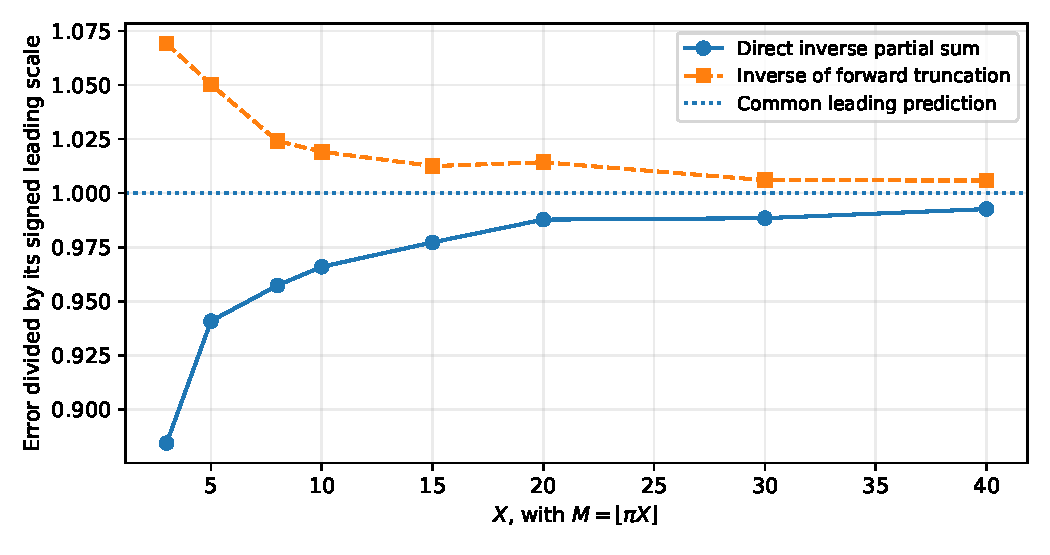
\includegraphics[width=0.93\linewidth]{figures/direct_vs_forward.pdf}
\caption{Recorded high-precision errors divided by
$(-1)^M\sqrt X\ee^{-2\pi X}$, with $M=\lfloor\pi X\rfloor$.
Both curves tend to one, but their first corrections differ. The oscillation caused by the bounded shift $\sigma$ is retained rather than smoothed away.}
\label{fig:comparison}
\end{figure}

\section{A cosine representation of the inverse Borel transform}
\label{sec:borel}

\subsection{An elementary representation and positive-direction summation}
For a formal series $\sum_{m\ge1}a_mX^{-m}$, use the ordinary Borel transform at infinity
\[
 \Borel\left(\sum_{m\ge1}a_mX^{-m}\right)(\xi)
 =\sum_{m\ge1}\frac{a_m}{\Gamma(m)}\xi^{m-1}.
\]
In particular, for $U=W-X$ its formal transform is
\begin{equation}
 \widehat U(\xi)=\sum_{n\ge1}
                  \frac{h_n}{\Gamma(2n-1)}\xi^{2n-2}.
 \label{eq:Borel-series}
\end{equation}

\begin{theorem}[Inverse cosine transform]
\label{thm:borel}
The Borel series \eqref{eq:Borel-series} converges near zero and has the analytic continuation
\begin{equation}
 \widehat U(\xi)=\widehat E_R(\xi)
              -\frac2\pi\int_R^\infty\rho(t)\cos(t\xi)\,\dd t,
 \qquad |\Im\xi|<2\pi,
 \label{eq:cosine}
\end{equation}
where
\begin{equation}
 \widehat E_R(\xi)=\sum_{n\ge1}
              \frac{e_n}{(2n-2)!}\xi^{2n-2}
 \label{eq:Ehat}
\end{equation}
is entire of exponential type at most $R$. For real $X>R$,
\begin{equation}
 \int_0^\infty\ee^{-X\xi}\widehat U(\xi)\,\dd\xi=W(X)-X.
 \label{eq:Borel-sum}
\end{equation}
Thus the formal inverse is Borel-summed in the positive direction by the actual exterior inverse.
\end{theorem}
\begin{proof}
Bound \eqref{eq:e-bound} gives
$|\widehat E_R(\xi)|\le K_R\ee^{R|\xi|}$. By \cref{thm:density}, the integral in \eqref{eq:cosine} converges absolutely and locally uniformly in the stated strip. Near zero, expansion of the cosine under the integral is justified on every smaller disk of radius less than $2\pi$. Its coefficient of $\xi^{2n-2}$ is
\[
 -\frac2\pi\frac{(-1)^{n-1}}{(2n-2)!}
                 \int_R^\infty\rho(t)t^{2n-2}\,\dd t,
\]
which agrees with \eqref{eq:Borel-series} by \eqref{eq:h-moment}. This proves both local convergence and continuation.

On the positive real ray the spectral part of \eqref{eq:cosine} is bounded, and the entire part has at most exponential growth $\ee^{R\xi}$. Its Laplace integral therefore converges for $X>R$. Absolute Fubini is valid for the spectral part since $\rho$ is integrable and $|\cos(t\xi)|\le1$ for real arguments. The elementary integral
\[
 \int_0^\infty\ee^{-X\xi}\cos(t\xi)\,\dd\xi
       =\frac{X}{X^2+t^2}
\]
and termwise Laplace integration of \eqref{eq:Ehat} recover \eqref{eq:spectral}. This proves \eqref{eq:Borel-sum}.
\end{proof}

Positive-direction summability was already obtained in the repository from general nonlinear closure \cite{prior,sauzin}. The contribution of \cref{thm:borel} is an explicit inverse cosine representation and a direct proof from the same spectral density that controls real remainders. The theorem makes no use of a full resurgent continuation theorem.

\subsection{Nearest boundary singularities, including logarithmic terms}
Let $a=2\pi$. Near the upper boundary point $\xi=\ii a$, put
\begin{equation}
 q=a+\ii\xi.
 \label{eq:q-upper}
\end{equation}
An inward approach means $q\to0$ through $\Re q>0$. To state uniform asymptotics, restrict $q$ to any closed cone
$|\arg q|\le\pi/2-\delta$, with fixed $\delta>0$, and use the logarithm in the right half-plane.

\begin{theorem}[Complete one-sided singular expansion]
\label{thm:boundary}
For every integer $L\ge0$, there is a polynomial $Q_L$ of degree at most $L$ such that, in each inward cone,
\begin{align}
 \widehat U(\xi)={}&-\frac1{q^2}-\frac{d_1}{q}
   +\sum_{m=2}^{L+2}
       \frac{(-1)^{m-2}d_m}{(m-2)!}\,q^{m-2}\log q
   +Q_L(q)+o(|q|^L),
 \label{eq:boundary-all}
\end{align}
where $q=a+\ii\xi$. In particular,
\begin{equation}
 \widehat U(\xi)=\frac1{(\xi-2\pi\ii)^2}
 -\frac{\pi\ii}{12(\xi-2\pi\ii)}
 +\frac{\pi^2-12}{288}\log(2\pi+\ii\xi)+\Oh(1).
 \label{eq:boundary-first}
\end{equation}
At $-2\pi\ii$ the expansion is its complex conjugate, with
$q=2\pi-\ii\xi$ and simple-pole coefficient $+\pi\ii/12$.
The Taylor radius of \eqref{eq:Borel-series} is exactly $2\pi$, and the nearest boundary singularities are not meromorphic singularities.
\end{theorem}
\begin{proof}
Split the cosine into its two exponentials. Near the upper boundary point, the term containing $\ee^{\ii t\xi}$ still decays at a rate close to $2a$ and is holomorphic in a neighborhood of that point. The potentially singular term is
\begin{equation}
 -\frac1\pi\int_R^\infty\rho(t)\ee^{-\ii t\xi}\,\dd t.
 \label{eq:singular-half}
\end{equation}
Substitute the density expansion through $d_{L+2}$. Because
$\rho(t)/\pi=\ee^{-at}\sum_{m=0}^{L+2}d_mt^{1-m}
+\Oh(\ee^{-at}t^{-L-2})$, the remainder in \eqref{eq:singular-half} has $L$ continuous derivatives at $q=0$ from the closed right half-plane. Indeed, after $k\le L$ derivatives its integrand is bounded by a constant times $t^{k-L-2}$, an integrable function. Its Taylor polynomial of degree $L$ therefore leaves $o(|q|^L)$ uniformly in the indicated cones.

It remains to expand the elementary integrals
\[
 I_m(q)=\int_R^\infty t^{1-m}\ee^{-qt}\,\dd t.
\]
For $m=0,1$, their singular parts are $q^{-2}$ and $q^{-1}$. For $m=2$,
$I_2(q)=-\log q$ plus a function holomorphic at zero. For larger $m$, the identity $I_m'(q)=-I_{m-1}(q)$ yields recursively the singular part
\[
 \frac{(-1)^{m-1}}{(m-2)!}\,q^{m-2}\log q.
\]
Multiplication by $-d_m$ in \eqref{eq:singular-half}, followed by absorption of all regular Taylor terms into $Q_L$, proves \eqref{eq:boundary-all}. The entire function $\widehat E_R$ contributes only to that regular polynomial.

Formula \eqref{eq:boundary-first} follows from $q=\ii(\xi-\ii a)$ and \eqref{eq:d-first}. Conjugation of \eqref{eq:cosine} gives the lower-boundary statement. The strip representation gives a Taylor radius at least $a$; the nonzero double-pole leading behavior at distance $a$ gives the reverse inequality. Finally, $(\pi^2-12)/288\ne0$. After the double and simple poles have been subtracted, the residual logarithmic divergence cannot be the restriction of a holomorphic function at the point. No meromorphic local extension can therefore account for the boundary behavior.
\end{proof}

\begin{remark}[The precise boundary of this answer]
Equation \eqref{eq:boundary-all} determines every logarithmic coefficient and both pole coefficients in a one-sided singular expansion. The regular polynomials $Q_L$ depend on global data. The statement is not, by itself, an assertion that the infinite singular expansion converges, a construction of continuation around the singular point, or a classification of every subsequent Borel sheet. Those stronger questions require more than the Abelian boundary argument used here. This distinction prevents an explicit boundary expansion from being misrepresented as a complete resurgent singular-germ theorem.
\end{remark}

\subsection{Why the inner correction cannot change these singular coefficients}
The Borel transform of any geometrically bounded Laurent coefficient sequence is entire. All dependence of $E_R$ on the fixed inner disk therefore lies in an entire Borel function. The pole and logarithmic coefficients in \eqref{eq:boundary-all} depend only on the large-$t$ tail of $\rho$. This cleanly separates finite-region analytic information from the late-coefficient and nearest-singularity information. It also makes cutoff invariance transparent.

\section{A general reflection-to-inversion transfer theorem}
\label{sec:general}

The preceding construction uses two different kinds of information. The exterior logarithmic asymptotic expansion gives a well-defined inverse and bounds its derivatives. The boundary-phase defect supplies the exponentially small density. The following theorem isolates that mechanism without referring to the special-function identity that generated the defect.

\begin{theorem}[Boundary-phase transfer]
\label{thm:transfer}
Let $F$ be holomorphic on an exterior sector containing a neighborhood of the closed right half-plane. Suppose the following conditions hold.
\begin{enumerate}[label=\textup{(\roman*)},leftmargin=2em,itemsep=3pt]
\item $F$ respects conjugation, and has the uniform, differentiable expansion
\[
 F(w)\sim\log w+\sum_{j\ge1}c_jw^{-2j},\qquad c_j\in\R.
\]
In particular, $F'=w^{-1}+\Oh(w^{-3})$ and $F''=\Oh(w^{-2})$ on smaller sectors.
\item For $v>0$ large, $F(\ii v)=A(v)+\ii(\pi/2-J(v))$, where $A,J$ are real, $J(v)>0$, and
\begin{equation}
 J(v)=\kappa v^\beta\ee^{-av}(1+\Oh(v^{-1})),\qquad
 J'(v)=\Oh(v^\beta\ee^{-av}),
 \label{eq:general-defect}
\end{equation}
with $a,\kappa>0$ and fixed $\beta\in\R$.
\end{enumerate}
Let $W$ be the exterior inverse of $F(W(X))=\log X$, and write its formal expansion as $X+\sum h_nX^{1-2n}$. Then for large $t$,
\begin{equation}
 -\Re W(\ii t)=\kappa t^{\beta+1}\ee^{-at}(1+\Oh(t^{-1}))>0.
 \label{eq:general-density}
\end{equation}
An exact spectral decomposition and convergent core of the form \eqref{eq:spectral} exist. Consequently,
\begin{equation}
 h_n\sim\frac{2\kappa}{\pi}(-1)^n
                \frac{\Gamma(2n+\beta)}{a^{2n+\beta}},
 \label{eq:general-late}
\end{equation}
and, whenever $M-aX/2$ stays bounded,
\begin{equation}
 S_M(X)-W(X)
 =(-1)^M\frac{\kappa}{\pi}\sqrt{\frac{2\pi}{a}}
           X^{\beta+1/2}\ee^{-aX}(1+\Oh(X^{-1})).
 \label{eq:general-optimal}
\end{equation}
There is also an eventual strict enveloping theorem uniform for $X\ge2R$ and all sufficiently large $M$, as in \cref{thm:enveloping}.
\end{theorem}
\begin{proof}
The contraction argument of \cref{lem:inverse} depends only on condition (i), so it supplies the required inverse branch and formal odd Laurent expansion. The real equation $A(v(t))=\log t$ gives $v=t+\Oh(t^{-1})$ and $A'(v)\sim1/v$. Its target value differs from $\log(\ii t)$ by $\ii J(v)$. The same local inverse calculation as in \eqref{eq:delta} gives
\[
 -\Re W(\ii t)
 =\frac{J(v)A'(v)}{A'(v)^2+J'(v)^2}+\Oh(vJ(v)^2).
\]
The derivative assumption in \eqref{eq:general-defect} makes $J'/A'$ exponentially small. Thus the right side is asymptotic to
$\kappa v^{\beta+1}\ee^{-av}$, and replacing $v$ by $t+\Oh(t^{-1})$ proves \eqref{eq:general-density} with its error. The sign is eventually positive.

The piecewise exterior function and Cauchy proof use only conjugation, the $\Oh(1/z)$ decay, and the exponentially decaying jump, so \eqref{eq:spectral} holds unchanged. Its coefficient moments and \eqref{eq:general-density} yield \eqref{eq:general-late}; the correction from a relative $\Oh(t^{-1})$ in the density has relative size $\Oh(n^{-1})$ in that moment.

For the direct remainder, replace $\rho(t)$ by its leading form in \eqref{eq:exact-remainder}. Put $s=2M+\beta+2$ and $b=aX$, so $s-b$ remains bounded. The positive integral has leading value
\[
 \kappa\frac{\Gamma(s)}{a^s}\E f(U_s/b)
 =\frac\kappa2\frac{\Gamma(s)}{a^s}(1+\Oh(X^{-1})).
\]
After multiplication by $2/(\pi X^{2M+1})$ and application of shifted Stirling, this is
$(\kappa/\pi)\sqrt{2\pi/a}\,X^{\beta+1/2}\ee^{-aX}
(1+\Oh(X^{-1}))$. The convergent core is superexponentially smaller on this scale. This proves \eqref{eq:general-optimal}.

For the eventual envelope, use the lower bound
$\rho(t)\ge c t^{\beta+1}\ee^{-at}$ in the proof of \cref{thm:enveloping}, with gamma shape $2M+\beta+2$. This shape is positive for all sufficiently large $M$, and its factorial growth still dominates the geometric core bound uniformly for $X\ge2R$. The same consecutive-sign argument completes the proof.
\end{proof}

\begin{remark}[The transfer theorem is conditional, not universal]
The hypotheses require a single positive, asymptotically specified phase defect and an exterior logarithmic inverse with real even-power corrections. They do not describe arbitrary resurgent implicit functions, sign-changing mixtures of actions, or a system with accumulating singular directions. Checking these hypotheses for another family is a mathematical task, not a notational substitution. For the centered digamma function, they are explicitly verified by \eqref{eq:phase-defect}, with $\kappa=\pi$, $a=2\pi$, and $\beta=0$.
\end{remark}

If the defect in \eqref{eq:general-defect} has a full inverse-power expansion with corresponding analytic derivative control, the argument gives all algebraic corrections to \eqref{eq:general-optimal}. One first calculates the amplitude of $-\Re W(\ii t)$ by local inverse Taylor expansion and then repeats the finite gamma-moment algorithm. This extension does not require positivity of every coefficient in that amplitude; only the eventual positivity of the density is used for enveloping.

\section{Reproducible computations and independent checks}
\label{sec:computation}

\subsection{What the programs check}
The archive contains exact rational coefficient calculations, high-precision real and complex evaluations, and a separate finite-quadrature test of the contour identity. None of these numerical tests is used as a substitute for the all-orders proofs.

The exact part of \path{verification/verify.py} generates $h_1,\ldots,h_{14}$ with rational arithmetic. It verifies the defining formal residual through degree eight, generates $d_0,\ldots,d_6$ symbolically in $a$, and independently obtains \eqref{eq:B1}--\eqref{eq:B2} from the gamma-moment prescription. A separate 240-decimal-digit coefficient calculation is compared with the rational values through order fourteen. The higher-precision calculation then provides the coefficients needed through order 129 for the remainder tests.

For $X\in\{3,5,8,10,15,20,30,40\}$ and
$M=\lfloor\pi X\rfloor-1,\lfloor\pi X\rfloor,\lfloor\pi X\rfloor+1$,
the code evaluates the true inverse, the direct sum, and the inverse of the forward truncation. All twenty-four tested direct errors have the proved eventual sign. The tests at small $X$ are additional finite evidence, not a proof that the existential threshold in \cref{thm:enveloping} is below those values.

The inverse is selected numerically by Newton iteration starting from $X-1/(24X)$, also for complex $X=\ii t$. At 240 digits, the density evaluations for $t\le40$ still have ample precision to resolve the exponentially small real part, which is of order $\ee^{-2\pi t}$. Merely evaluating the imaginary part of the inverse to ordinary double precision would not resolve this density.

\subsection{Direct-remainder and separation data}
Define the normalized quantities
\begin{align}
 \mathcal R(X,M)&=\frac{S_M(X)-W(X)}{(-1)^M\sqrt X\ee^{-2\pi X}},\notag\\
 \mathcal D(X,M)&=\frac{S_M(X)-u_M(X)}
              {(-1)^{M+1}\pi\ee^{-2\pi X}/(6\sqrt X)}.
 \label{eq:numeric-ratios}
\end{align}
\Cref{tab:direct} records $\mathcal R$, the prediction
$1+B_1(\sigma)/X+B_2(\sigma)/X^2$, and $\mathcal D$, for the central truncation choice. The full-precision outputs and the neighboring orders are in \path{data/results.json} and \path{data/direct_remainders.csv}.

\begin{table}[htbp]
\centering\small
\begin{tabular}{rrrrr}
\toprule
$X$ & $M$ & Direct ratio & Two-correction prediction & Difference ratio \\
\midrule
3 & 9 & 0.884384132 & 0.885755655 & 1.058720318 \\
5 & 15 & 0.940788532 & 0.941014341 & 1.045230998 \\
8 & 25 & 0.957322610 & 0.957381115 & 1.020066135 \\
10 & 31 & 0.965933363 & 0.965956404 & 1.016339718 \\
15 & 47 & 0.977226495 & 0.977235012 & 1.010632293 \\
20 & 62 & 0.987744918 & 0.987748000 & 1.013099108 \\
30 & 94 & 0.988411034 & 0.988411959 & 1.005110173 \\
40 & 125 & 0.992624702 & 0.992624993 & 1.005188566 \\
\bottomrule
\end{tabular}

\caption{Actual recorded 240-digit calculations, displayed to nine decimal places. The last column tends to one as predicted by the direct-versus-forward separation theorem. Its nonmonotonicity is consistent with the varying bounded shift $\sigma$.}
\label{tab:direct}
\end{table}

\subsection{Density and contour checks}
The density calculation is checked against both the inverse-power amplitude and the independently computed linearized phase expression
$\pi\ee^{-2\pi v}/A'(v)$. The latter check tests the reflection-based mechanism directly, rather than only its first few formal coefficients. \Cref{fig:density} shows the amplitude comparison; the underlying data are in \path{data/density.csv}.

\begin{figure}[htbp]
\centering
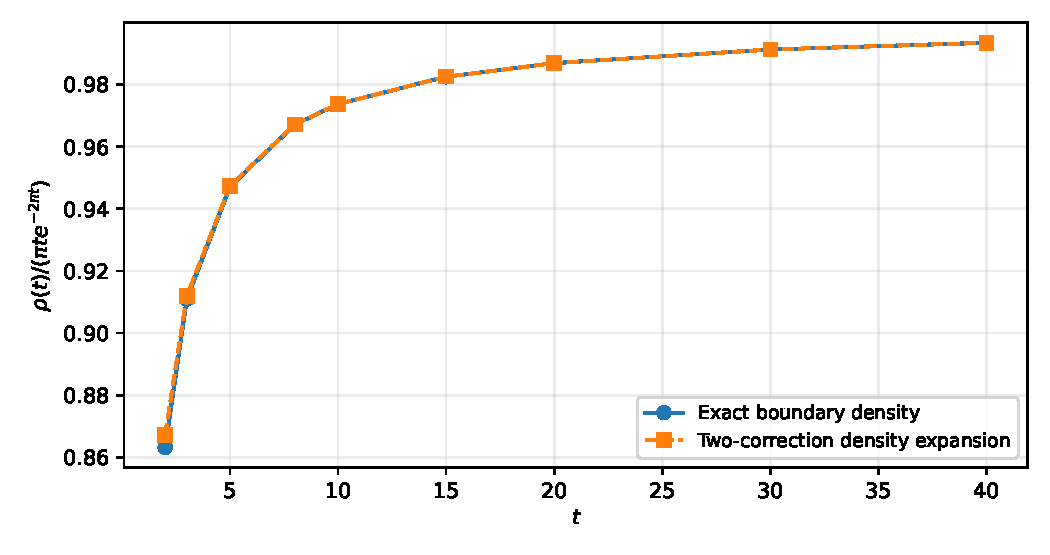
\includegraphics[width=0.93\linewidth]{figures/spectral_density.pdf}
\caption{The exact numerical density amplitude and
$1-\pi/(12t)+(\pi^2/288-1/24)t^{-2}$. Positivity at these finite inputs is observed numerically; eventual positivity for all sufficiently large inputs is proved in \cref{thm:density}.}
\label{fig:density}
\end{figure}

A separate program, \path{verification/contour_check.py}, uses the quarter-circle form of the inner-core tail:
\begin{equation}
 \mathcal E_{R,M}(X)=\frac{2}{\pi X^{2M+1}}\Re
 \int_0^{\pi/2}
 \frac{(W(\zeta)-\zeta)\zeta^{2M+1}}{1-(\zeta/X)^2}\,\dd\theta,
 \qquad \zeta=R\ee^{\ii\theta}.
 \label{eq:quarter-core}
\end{equation}
This follows from oddness and conjugation in the contour formula. At $R=2$, $X=5$, and $M=15$, the 100-digit, 36-node-per-interval calculation gives
\begin{align}
 \mathcal E_{R,M}(X)&\approx2.39942008131785481847\times10^{-19},\notag\\
 \text{spectral remainder}&\approx4.77761662822833134457\times10^{-14},\notag\\
 W(X)-S_M(X)&\approx4.77764062242914452311\times10^{-14}.
 \label{eq:contour-numbers}
\end{align}
The relative discrepancy in \eqref{eq:exact-remainder} is about
$5.4\times10^{-25}$. A lower 20-node calculation is also retained and is less accurate, illustrating the need to check quadrature resolution. The integration is cut off at $t=20$, and this diagnostic does not attach a rigorous quadrature or tail bound. It is an independent numerical check of orientation, normalization, and the nonzero core term, not a certificate of the identity or of a globally admissible cutoff $R=2$.

\subsection{Numerical evidence versus proof}
The universal assertions in this article follow from the exterior inverse construction, reflection identity, Cauchy representation, finite geometric identity, and uniform gamma estimates. The numerical programs check finite consequences and are intended to make sign or normalization mistakes detectable. They do not implement outward-rounded interval arithmetic, prove a global branch domain, certify every displayed digit, or mechanically verify the analytic proof. These boundaries are also stated in the output files.

\section{Further research questions and proposed next steps}
\label{sec:questions}

\begin{problem}[Effective and global enveloping thresholds]
Find explicit admissible constants $R$ and $M_0$ in \cref{thm:enveloping}; then determine the largest real domain and smallest truncation orders on which strict enveloping holds.
\end{problem}
The proof reduces the question to effective lower bounds for the phase-induced density and an upper bound on the inner contour. A successful result would separate a finite, certifiable parameter region from the factorial-dominance tail. It should not replace the inner correction by zero without a global inverse theorem. A counterexample at small argument or small order would be equally informative about the correct optimal statement.

\begin{problem}[Full local Borel germs and continuation sheets]
Upgrade the one-sided expansions in \cref{thm:boundary} to explicit continued singular germs, determine their regular parts or suitable normalization invariants, and propagate the data to later points of $2\pi\ii\mathbb Z$.
\end{problem}
The pole and logarithmic coefficients are now constrained to every order by $d_j$. What is missing is a constructive continuation around the boundary singularities and control of its sheets. Matching the spectral description with the inverse Stokes-sector formulas already in the repository would provide a stringent nonlinear consistency test. The regular polynomials $Q_L$ show precisely where the local singular information ceases to determine the full germ.

\begin{problem}[Second and higher exponential layers of the density]
Resolve $\rho(t)$ beyond its complete first amplitude multiplying $\ee^{-2\pi t}$, with exact or exponentially accurate remainder blocks.
\end{problem}
The exact defect $\pi/(\ee^{2\pi v}+1)$ has further exponential terms, while nonlinear inversion of the boundary equation creates additional products and derivatives. Determining whether cancellations remove particular sectors, and deriving a controlled transseries in $\ee^{-2\pi t}$, would turn \eqref{eq:exact-remainder} into a hyperasymptotic inverse algorithm. Truncating finitely many $d_j$ only improves powers within the first exponential sector; it does not establish an $\ee^{-4\pi X}$ error.

\begin{problem}[Uniform complex transition and Stokes smoothing]
Extend the direct-remainder theorem to complex $X$ approaching a Stokes direction at its natural transition scale, with a uniform terminant or error-function description.
\end{problem}
The exact spectral formula is already analytic in the right exterior domain. The denominator $X^2+t^2$ identifies where the saddle analysis interacts with a pole as the argument moves toward an imaginary direction. A correct theorem must track that interaction and the changing integration contour, rather than extrapolating the positive-real gamma estimate across a Stokes boundary.

\begin{problem}[Several phase defects and competing actions]
Generalize \cref{thm:transfer} to a finite collection of exponentially small boundary defects with different complex actions, including equal-modulus actions and cancellations.
\end{problem}
Positivity is the structural reason for eventual enveloping here. A signed or oscillatory density may retain an exact moment representation while losing the sign theorem. Useful criteria should distinguish cancellation of the leading late-coefficient contribution, removal of a nearest Borel singularity, and failure of real enveloping. These are related but not interchangeable phenomena.

\begin{problem}[The generalized-harmonic transition to $s=1$]
Develop a uniform direct-inverse remainder theory for
$H_s(x)=\zeta(s)-\zeta(s,x+1)$ as $s\downarrow1$ and $x\to\infty$ jointly.
\end{problem}
The companion volume treats fixed-parameter generalized harmonic inverses, and the earlier harmonic paper identifies the singular transition as open \cite{companion,prior}. A promising normalization should retain $(s-1)\log x$ and remove the artificial singularity caused by a fixed-$s$ endpoint coordinate. The challenge is to construct uniform boundary or spectral data that recover both the logarithmic harmonic limit and the fixed-$s$ inverse, with common remainder estimates.

\begin{problem}[Finite-region singularities and the convergent core]
Describe the analytic meaning of $E_R$ in terms of the finite critical values and singularities of the inverse, and determine whether a natural global spectral representation can absorb it.
\end{problem}
The present exterior approach intentionally avoids this classification. Since $E_R$ becomes an entire function after Borel transformation, it cannot alter the nearest factorial singular data, but it can determine low coefficients and small-argument behavior. Understanding it may settle global inequalities that are inaccessible from the asymptotic tail alone.

\begin{problem}[Other repository inverse families]
Identify gamma quotients or logarithmic inverse phases in the repository whose functional equations imply a positive boundary-phase defect satisfying \cref{thm:transfer}.
\end{problem}
The payoff would be an exact leading optimal-truncation constant and eventual direct envelopes without repeating the entire digamma proof. Each candidate needs a separately checked analytic exterior domain, differentiated asymptotic expansion, and defect asymptotic. Families with nonlogarithmic dominant cores may require a preliminary exact change of phase coordinate rather than a direct use of the theorem.

\begin{problem}[Formalization and certified complexity]
Formalize the finite moment and remainder identities first, then connect validated contour or spectral quadrature to a certified direct-inverse evaluator.
\end{problem}
The finite geometric identity, gamma moment polynomials, coefficient recurrences, and factorial-versus-geometric comparison have a relatively small proof-assistant dependency footprint. The analytic branch construction and contour representation require a larger complex-analysis interface. A computational implementation should separately bound coefficient arithmetic, special-function evaluation, core quadrature, spectral quadrature, and tail errors. The current scripts are transparent consistency tests, not such a verified evaluator.

\section{Synthesis}
\label{sec:conclusion}

A sharp direct-inverse remainder requires information that is absent from fixed-order reversion and from the leading growth of its coefficients alone. For the centered inverse digamma function, that information is encoded in the exponentially small phase mismatch of the forward function on the imaginary axis. The reflection identity makes the mismatch explicit. Local inversion turns it into a positive boundary density; an exterior Cauchy formula turns the density into an exact spectral decomposition; and a finite geometric identity turns that decomposition into the direct-truncation remainder.

This chain of arguments resolves the repository's direct-inverse optimal-truncation question in a precisely stated large-variable regime and proves a uniform eventual envelope beyond the least-term diagonal. It also identifies a concrete difference between direct summation and forward-truncation inversion at the first relative order, and yields all logarithmic coefficients of the nearest one-sided inverse-Borel singular expansions. The general transfer theorem shows that the mechanism is not tied to a single coefficient formula.

The remaining questions are genuinely additional: effective global thresholds, full Borel continuation sheets, higher exponential blocks, complex transition layers, and uniform parameter limits. None is used as an unproved premise in the results established here.

\appendix
\section{Coefficient and moment algorithms}
\label{app:algorithms}

\subsection{Exact inverse coefficients}
For fixed $q$ and $E(z)=\exp(q\cformal(z))=\sum E_kz^k$, differentiation gives
\begin{equation}
 E_0=1,\qquad
 E_k=\frac qk\sum_{j=1}^k j c_jE_{k-j}.
 \label{eq:E-recurrence}
\end{equation}
With $q=2n-1$, this computes $h_n=-E_n/q$. It uses exact rational arithmetic because each $c_j$ is rational. For one coefficient $h_n$, the displayed implementation takes quadratically many rational operations; calculating all coefficients by independently repeating it is cubic in the maximum order. No optimal bit-complexity claim is made.

\subsection{Density amplitude coefficients}
For compactness retain $a$ as a symbolic constant in \eqref{eq:d-algorithm}, while keeping the digamma values of $h_n$. The first terms beyond \eqref{eq:d-first} are
\begin{align}
 d_1&=-\frac a{24},&
 d_2&=\frac{a^2-48}{1152},\notag\\
 d_3&=-\frac{a(5a^2+1224)}{414720},&
 d_4&=\frac{5a^4+6336a^2-559872}{39813120},\notag\\
 d_5&=-\frac{a(7a^4+23856a^2+12342528)}{6688604160}.
 \label{eq:d-more}
\end{align}
Here $a=2\pi$ is substituted for the actual harmonic problem. Treating $a$ symbolically in this finite calculation is a bookkeeping device; it does not assert the existence of a family of digamma reflection identities with arbitrary action $a$.

To compute $d_j$, only finitely many $h_n$ enter. Set $z=1/t$, expand
\[
 \left(1-\sum_{n\ge1}(2n-1)(-1)^nh_nz^{2n}\right)
 \exp\left(-a\sum_{n\ge1}(-1)^nh_nz^{2n-1}\right)
\]
to the desired degree. No infinite numerical sum of the divergent series $V$ is performed.

\subsection{Moment generation without numerical fitting}
For an expansion through $b^{-K}$ in \eqref{eq:B-algorithm}, it is enough to use density terms $0\le j\le K$, the shifted Stirling exponent through $r=K$, and sufficiently many Taylor terms of $f$ at one. The exact moment polynomial \eqref{eq:moments} makes every operation algebraic. Taylor's theorem and the gamma even-moment bound are what justify truncating this finite calculation. Merely expanding a few moments without those bounds would not prove an all-orders remainder theorem.

The symbolic code verifies \eqref{eq:B1} by comparing the independently generated result to the displayed formula. It exports \eqref{eq:B2} as both a symbolic expression and its LaTeX form. The numerical evaluator then uses that generated expression, rather than a separately hard-coded polynomial, for the two-correction prediction in \cref{tab:direct}.

\section{Reproduction and provenance}
\label{app:provenance}

\subsection{Rebuilding the package}
The archive is self-contained and does not require repository-relative notation files. From its top-level directory, run
\begin{verbatim}
python verification/verify.py
python verification/contour_check.py
python verification/make_figures.py
pdflatex -interaction=nonstopmode -halt-on-error \
  inverse_digamma_spectral.tex
pdflatex -interaction=nonstopmode -halt-on-error \
  inverse_digamma_spectral.tex
\end{verbatim}
The stored data and figures permit rebuilding the article without rerunning the numerical tests. The Python programs use SymPy, mpmath, and matplotlib. Their recorded version numbers are in \path{data/results.json}. A normal LaTeX installation with the packages in the preamble, including \texttt{newtxtext} and \texttt{newtxmath}, is required. Font files are not distributed.

\subsection{The inspected repository checkpoint}
The repository checkpoint used for the final source identification is
\begin{center}\small
\texttt{5804c7aff9955e6cbc09be2a71a295a07b238bc9}.
\end{center}
The central source was
\begin{quote}\small\raggedright
\path{Analysis/Transseries/docs/series-and-transseries/Inverse_Harmonic_Stokes_Transport/inverse_harmonic_transseries.tex}.
\end{quote}
Its Git blob is
\texttt{2da951cd1d724042f9784365a448c584984ece74}.
The inspected source portions include its normalization and coefficient formula, its sharp forward-truncation-inverse analysis, Borel discussion, and research questions. The group README was inspected to establish the distinction between the canonical volume, the combinatorial companion, and recent unmerged research packages.

The canonical and companion paths at this checkpoint are
\begin{quote}\small\raggedright
\path{Analysis/Transseries/docs/series-and-transseries/Transseries_And_Inversion/transseries_and_inversion.tex},\par
\path{Analysis/Transseries/docs/series-and-transseries/Combinatorial_Transseries_Inverses/Combinatorial_Transseries_Inverses.tex}.
\end{quote}
Earlier repository manuscripts refer to pre-split paths under
\path{Analysis/FabiusFunction/docs/semi-formalized-research-frontiers/drafts/series-and-transseries/}. Those older paths in their bibliographies should not be confused with the locations inspected here.

The checkpoint also contains newly arrived binary research archives. They were not unpacked and audited claim by claim in this work. Accordingly, the novelty comparison here is against the identified filed manuscripts and the public literature checked, not an exhaustive assertion about every artifact in the repository or every concurrent research draft.

\subsection{Audit ledger}
\begin{longtable}{@{}>{\raggedright\arraybackslash}p{0.26\linewidth}>{\raggedright\arraybackslash}p{0.68\linewidth}@{}}
\toprule
Claim or artifact & Verification status\\
\midrule
\endhead
Exterior inverse, density, contour representation & Conventional proofs in \cref{sec:inverse,sec:density,sec:spectral}; no global inverse theorem assumed.\\[3pt]
Direct all-orders remainder and eventual envelopes & Conventional proofs in \cref{sec:remainder,sec:optimal}; thresholds are not numerically certified.\\[3pt]
Nearest Borel boundary data & One-sided all-orders singular expansion in \cref{thm:boundary}; not a complete continuation-sheet construction.\\[3pt]
Finite coefficients and error polynomials & Exact rational/symbolic checks in the included program.\\[3pt]
Real and complex numerical values & 240-digit mpmath tests; no interval certification.\\[3pt]
Contour identity diagnostic & Independent 100-digit finite quadrature, with both lower and higher quadrature orders retained.\\[3pt]
Existing coefficient asymptotics and summability & Credited to the earlier literature and repository; not advertised as new.\\[3pt]
Lean and global priority & Neither a new Lean proof nor an established worldwide priority claim is asserted.\\
\bottomrule
\end{longtable}

\clearpage
\begin{thebibliography}{9}
\addcontentsline{toc}{section}{References}

\bibitem{prior}
\emph{Exponential Accuracy and Stokes Transport for Inverse Harmonic Transseries}, research manuscript in Vladimir Reshetnikov's \repo\ repository, 29 September 2026. Inspected at commit
\texttt{5804c7aff9955e6cbc09be2a71a295a07b238bc9}; exact path and blob in \cref{app:provenance}. In particular, the research discussion explicitly leaves the sharp direct-inverse-partial-sum remainder open.
\url{https://github.com/VladimirReshetnikov/ProveIt/tree/5804c7aff9955e6cbc09be2a71a295a07b238bc9/Analysis/Transseries/docs/series-and-transseries/Inverse_Harmonic_Stokes_Transport}.

\bibitem{companion}
\emph{Combinatorial Transseries and Their Inverses: Gamma quotients, finite exponential sums, moment sectors, moving saddles, arithmetic sheets, and q-products}, companion manuscript in \repo\, same checkpoint. The harmonic coefficient formula and fixed-order inversion are the starting point of the preceding harmonic manuscript. Group organization and scope are documented in the adjacent README.
\url{https://github.com/VladimirReshetnikov/ProveIt/tree/5804c7aff9955e6cbc09be2a71a295a07b238bc9/Analysis/Transseries/docs/series-and-transseries}.

\bibitem{dlmf}
NIST Digital Library of Mathematical Functions, Chapter 5, especially \S5.5 (functional relations), \S5.9 (integral representations), and \S5.11 (asymptotic expansions), accessed 29 September 2026.
\url{https://dlmf.nist.gov/5.5};
\url{https://dlmf.nist.gov/5.9};
\url{https://dlmf.nist.gov/5.11}.

\bibitem{issaka}
Aziz Issaka, ``On Ramanujan's inverse digamma approximation,''
\emph{The Ramanujan Journal} \textbf{39} (2016), 291--302.
\url{https://doi.org/10.1007/s11139-014-9659-3}.

\bibitem{nemes}
Gerg\H{o} Nemes, ``Proofs of two conjectures on the real zeros of the cylinder and Airy functions,''
\emph{SIAM Journal on Mathematical Analysis} \textbf{53}(4) (2021), 4328--4349.
\url{https://doi.org/10.1137/21M1396794}.
Preprint: \url{https://arxiv.org/abs/2010.13069}.

\bibitem{borinsky}
Michael Borinsky, ``Generating asymptotics for factorially divergent sequences,''
\emph{Electronic Journal of Combinatorics} \textbf{25}(4) (2018), P4.1.
\url{https://doi.org/10.37236/5999}.
Preprint: \url{https://arxiv.org/abs/1603.01236}.

\bibitem{sauzin}
David Sauzin, ``Nonlinear analysis with resurgent functions,''
\emph{Annales scientifiques de l'\'Ecole normale sup\'erieure}, series 4,
\textbf{48}(3) (2015), 667--702.
\url{https://doi.org/10.24033/asens.2255}.
Preprint: \url{https://arxiv.org/abs/1212.4477}.

\end{thebibliography}
\end{document}
